\paragraph{Phân tích Dữ liệu (EDA)} \hfill \\
Trước khi huấn luyện, chúng ta quan sát sự phân bổ độ dài văn bản và các từ khóa đặc trưng của hai lớp cảm xúc.

\begin{figure}[H]
    \centering
    \begin{minipage}{0.48\textwidth}
        \centering
        
\includegraphics[width=\linewidth]{Chương_3/results/imdb_bigru/01_eda_overview.png}
        \caption{Phân bổ độ dài và thống kê từ vựng IMDB}
        \label{fig:imdb_eda}
    \end{minipage}
    \hfill
    \begin{minipage}{0.48\textwidth}
        \centering
        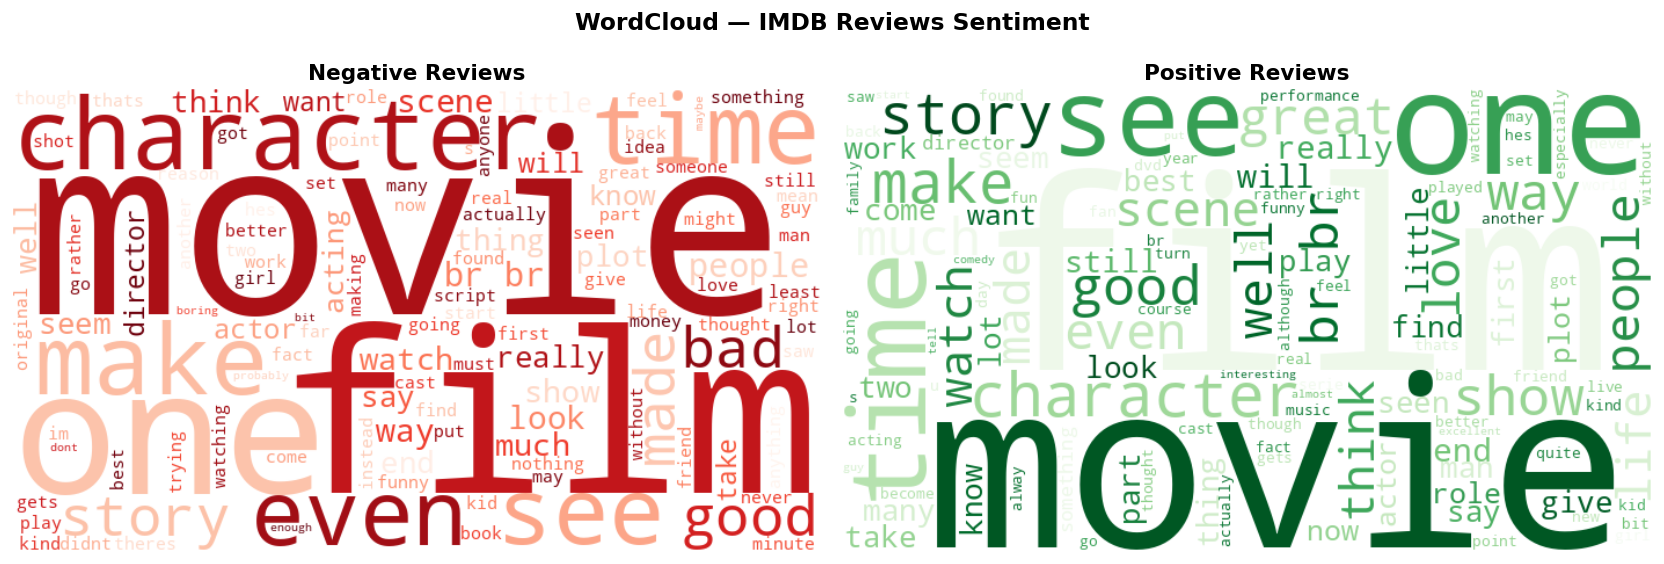
\includegraphics[width=\linewidth]{Chương_3/results/imdb_bigru/02_wordclouds.png}
        \caption{WordCloud các từ xuất hiện nhiều}
        \label{fig:imdb_wc}
    \end{minipage}
\end{figure}

\paragraph{Mô hình Bidirectional GRU} \hfill \\
Kiến trúc GRU hai chiều cho phép mô hình học thông tin từ cả hai hướng của câu văn, giúp nắm bắt ngữ cảnh tốt hơn. Mô hình sử dụng \textbf{2,099,073} tham số.

\paragraph{Kết quả huấn luyện và Phân tích} \hfill \\
Mô hình đạt độ chính xác ấn tượng là \textbf{86.67\%} với chỉ số \textbf{ROC-AUC là 0.9392}, vượt xa so với mạng RNN truyền thống.

\begin{figure}[H]
    \centering
    \begin{minipage}{0.48\textwidth}
        \centering
        
\includegraphics[width=\linewidth]{Chương_3/results/imdb_bigru/03_training_history.png}
        \caption{Lịch sử huấn luyện Bidirectional GRU}
        \label{fig:imdb_history}
    \end{minipage}
    \hfill
    \begin{minipage}{0.48\textwidth}
        \centering
        
\includegraphics[width=\linewidth]{Chương_3/results/imdb_bigru/04_confusion_roc.png}
        \caption{Confusion Matrix và Đường cong ROC}
        \label{fig:imdb_roc}
    \end{minipage}
\end{figure}

\begin{figure}[H]
    \centering
    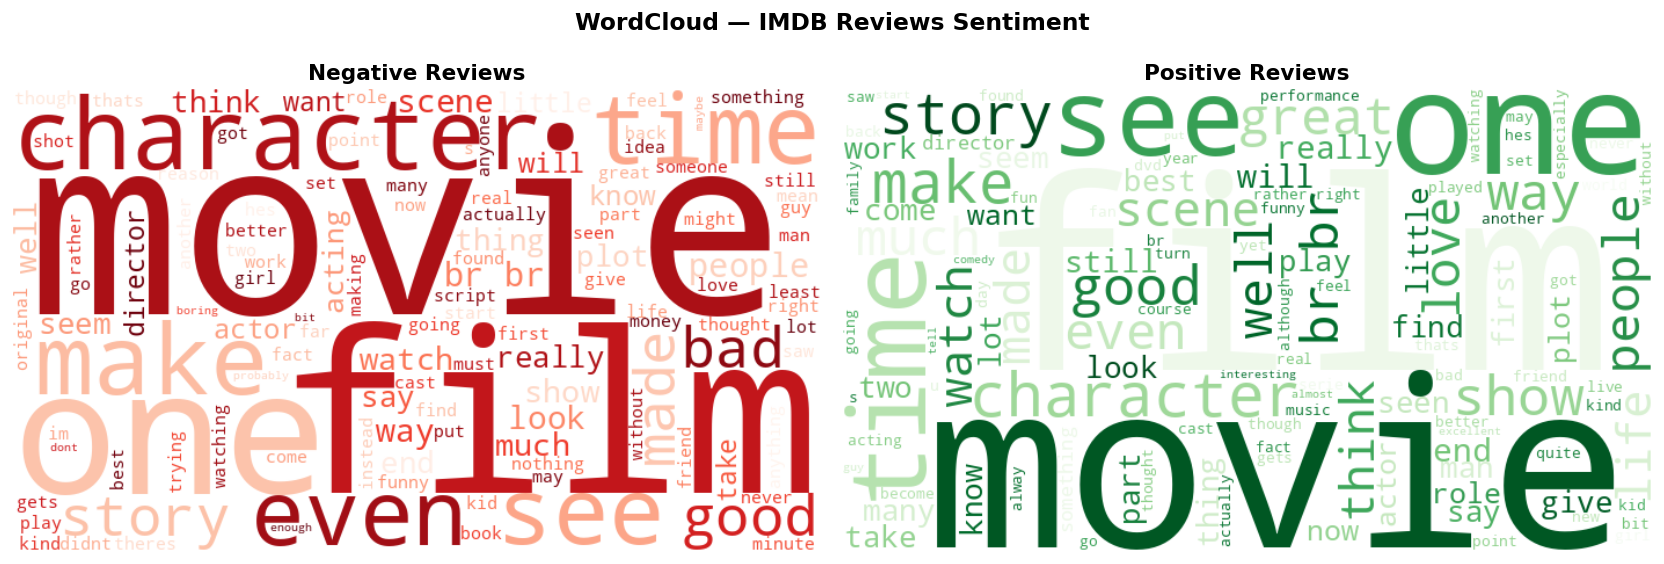
\includegraphics[width=0.8\linewidth]{Chương_3/results/imdb_bigru/02_wordclouds.png}
    \caption{WordCloud các từ xuất hiện nhiều trong đánh giá Tích cực và Tiêu cực}
    \label{fig:imdb_wc_large}
\end{figure}

Việc sử dụng kiến trúc hai chiều giúp GRU nhận diện được các sắc thái biểu cảm phức tạp trong các bài đánh giá phim dài.

\paragraph{Phụ lục: Quy trình thực nghiệm chi tiết} \hfill \\
Dưới đây là các bước triển khai chi tiết trên môi trường Jupyter Notebook:

\begin{figure}[H]
    \centering
    
\includegraphics[width=0.9\linewidth]{Chương_3/docs/ch3/17.png}
    \caption{Thiết lập môi trường: Cấu hình thư mục lưu trữ và Hyperparameters cho mô hình Bidirectional GRU.}
\end{figure}

\begin{figure}[H]
    \centering
    
\includegraphics[width=0.9\linewidth]{Chương_3/docs/ch3/18.png}
    \caption{Tải dữ liệu IMDB: Kiểm tra tính cân bằng của tập dữ liệu với 25,000 mẫu tích cực và 25,000 mẫu tiêu cực.}
\end{figure}

\begin{figure}[H]
    \centering
    
\includegraphics[width=0.9\linewidth]{Chương_3/docs/ch3/19.png}
    \caption{Mã nguồn EDA chuyên sâu: Tính toán phân bổ số lượng từ và phần trăm bao phủ của `MAX\_LEN`.}
\end{figure}

\begin{figure}[H]
    \centering
    
\includegraphics[width=0.9\linewidth]{Chương_3/docs/ch3/20.png}
    \caption{Kết quả EDA IMDB: Trực quan hóa cho thấy đa số các bài đánh giá có độ dài dưới 200 từ.}
\end{figure}

\begin{figure}[H]
    \centering
    
\includegraphics[width=0.9\linewidth]{Chương_3/docs/ch3/21.png}
    \caption{Làm sạch văn bản: Mã nguồn loại bỏ các thẻ HTML (nếu có) và chuẩn hóa văn bản cho WordCloud.}
\end{figure}

\begin{figure}[H]
    \centering
    
\includegraphics[width=0.9\linewidth]{Chương_3/docs/ch3/22.png}
    \caption{WordCloud cảm xúc: So sánh các từ khóa đặc trưng nhất của lớp Tích cực (xanh) và Tiêu cực (đỏ).}
\end{figure}

\begin{figure}[H]
    \centering
    
\includegraphics[width=0.9\linewidth]{Chương_3/docs/ch3/23.png}
    \caption{Kiến trúc Bi-GRU: Xây dựng mô hình sử dụng lớp `Bidirectional` bọc ngoài `GRU` để nắm bắt ngữ cảnh hai chiều.}
\end{figure}

\begin{figure}[H]
    \centering
    
\includegraphics[width=0.9\linewidth]{Chương_3/docs/ch3/24.png}
    \caption{Model Summary: Chi tiết số lượng tham số huấn luyện (hơn 2 triệu tham số).}
\end{figure}

\begin{figure}[H]
    \centering
    
\includegraphics[width=0.9\linewidth]{Chương_3/docs/ch3/25.png}
    \caption{Quá trình huấn luyện Bi-GRU: Mô hình hội tụ rất nhanh với độ chính xác trên tập Validation đạt trên 86\%.}
\end{figure}

\begin{figure}[H]
    \centering
    
\includegraphics[width=0.9\linewidth]{Chương_3/docs/ch3/26.png}
    \caption{Kết quả Training History: Đường cong Accuracy và Loss cho thấy mô hình không bị Overfitting nghiêm trọng.}
\end{figure}

\begin{figure}[H]
    \centering
    
\includegraphics[width=0.9\linewidth]{Chương_3/docs/ch3/27.png}
    \caption{Đánh giá tổng thể: Sự kết hợp giữa Ma trận nhầm lẫn và đường cong ROC minh chứng cho hiệu năng mạnh mẽ của GRU.}
\end{figure}

\begin{figure}[H]
    \centering
    
\includegraphics[width=0.9\linewidth]{Chương_3/docs/ch3/28.png}
    \caption{Inference Demo: Thử nghiệm dự báo trực tiếp trên các câu văn mới để kiểm tra tính thực tế của mô hình.}
\end{figure}
